% 表紙
\thispagestyle{empty}
\begin{tikzpicture}[remember picture,overlay]
  \fill[black!92] (current page.north west) rectangle (current page.south east);
  \node[anchor=north,inner sep=0pt] at ($(current page.north)+(0,-2.2cm)$)
    {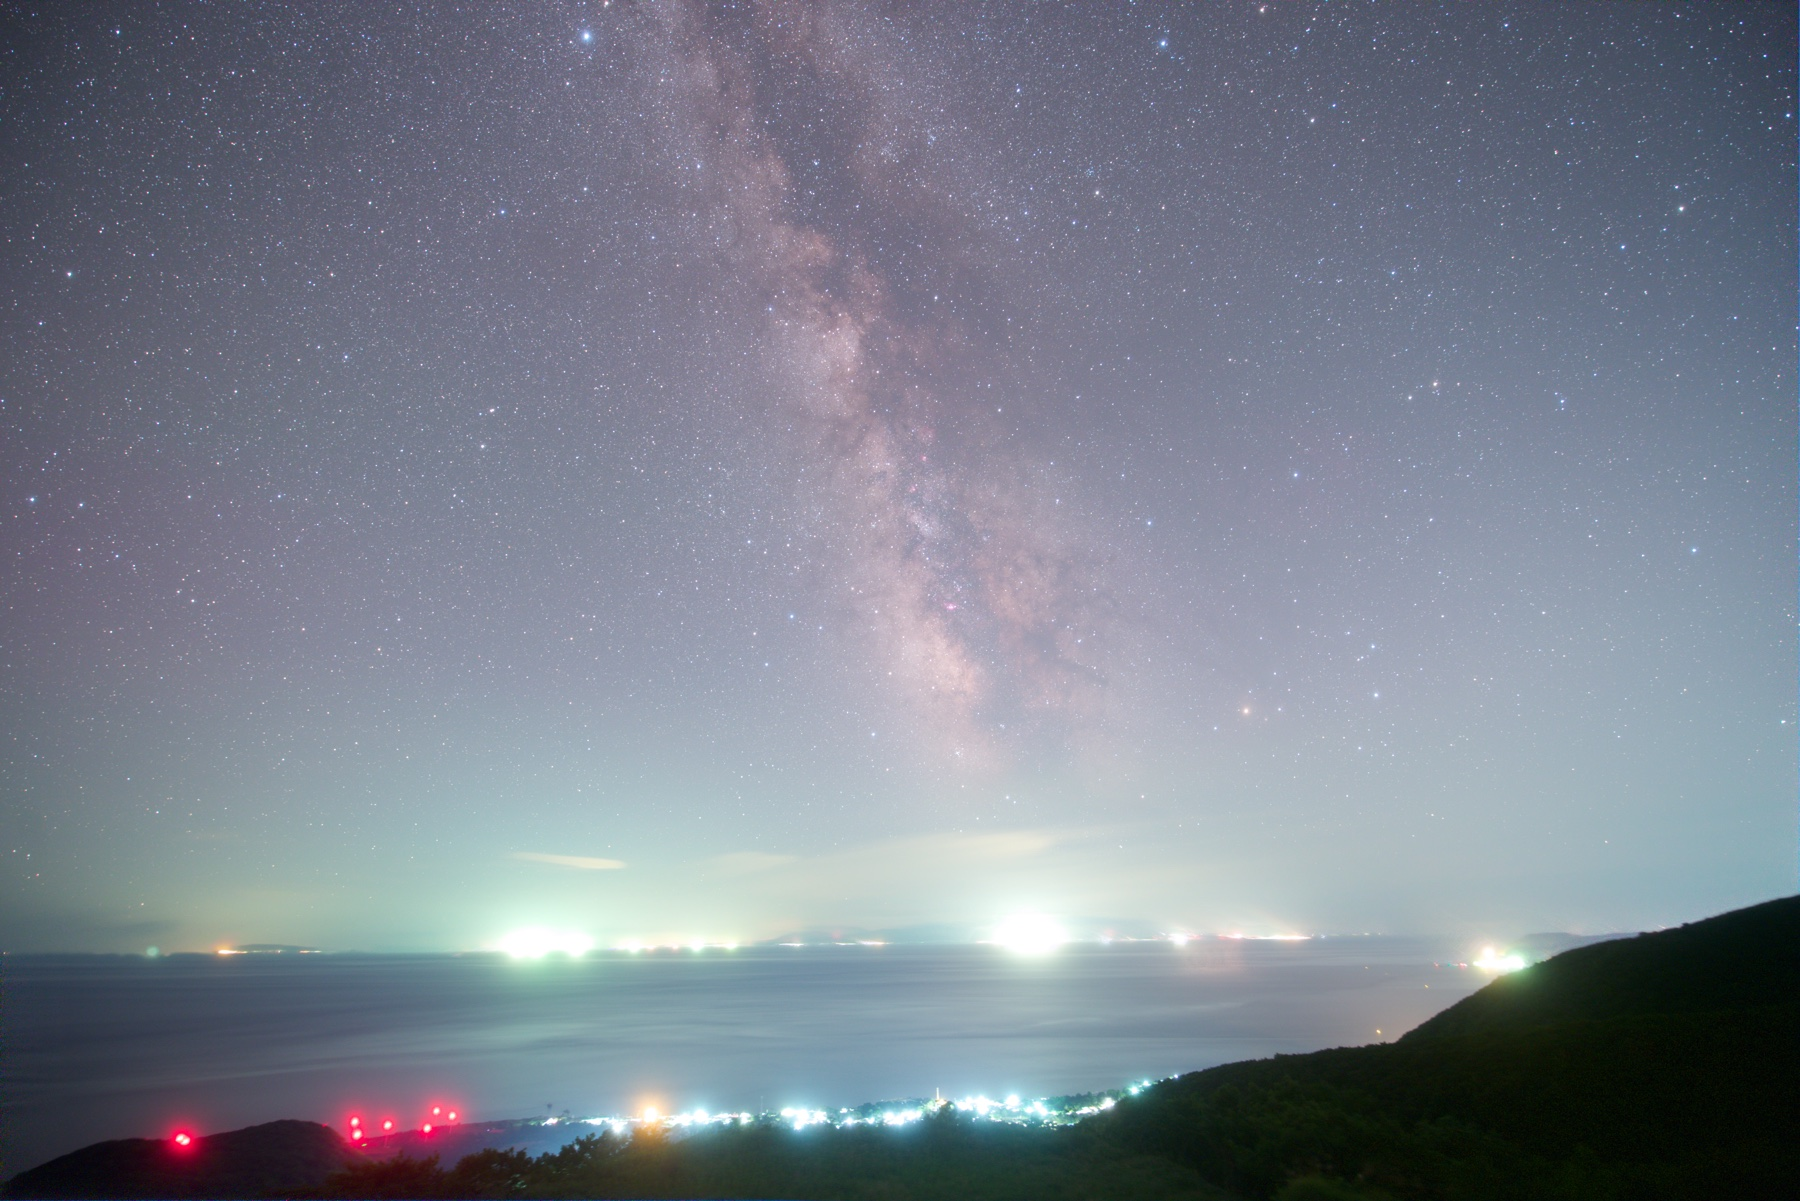
\includegraphics[width=0.86\paperwidth]{figures/photo_nightscape}};
  \node[anchor=north,text=white,font=\sffamily\bfseries\fontsize{30}{36}\selectfont]
    at ($(current page.north)+(0,-15.8cm)$) {MacStarStacker};
  \node[anchor=north,text=accent,font=\sffamily\bfseries\fontsize{20}{26}\selectfont]
    at ($(current page.north)+(0,-17.6cm)$) {使い方ガイド};
  \node[anchor=north,text=white!80,font=\sffamily\large,align=center]
    at ($(current page.north)+(0,-19.6cm)$) {星景写真のスタッキング（合成）アプリ\\[0.6ex]
      はじめての方でも、画面を見ながら順番に進められるように説明します};
  \node[anchor=south,text=white!70,font=\sffamily,align=center]
    at ($(current page.south)+(0,2.4cm)$) {バージョン 2.0\\[0.4ex]\small https://github.com/Geology-cat/MacStarStacker};
  \node[anchor=south east,text=white!55,font=\sffamily\scriptsize]
    at ($(current page.south east)+(-1.2cm,0.8cm)$) {表紙の写真：MacStarStacker の新星景モードで合成した例};
\end{tikzpicture}
\null
\clearpage
